\documentclass{standalone}
\usepackage{tikz}
\usetikzlibrary{patterns, positioning}
\usepackage[sfdefault]{ClearSans} %% option 'sfdefault' activates Clear Sans as the default text font
\usepackage[T1]{fontenc}

\begin{document}
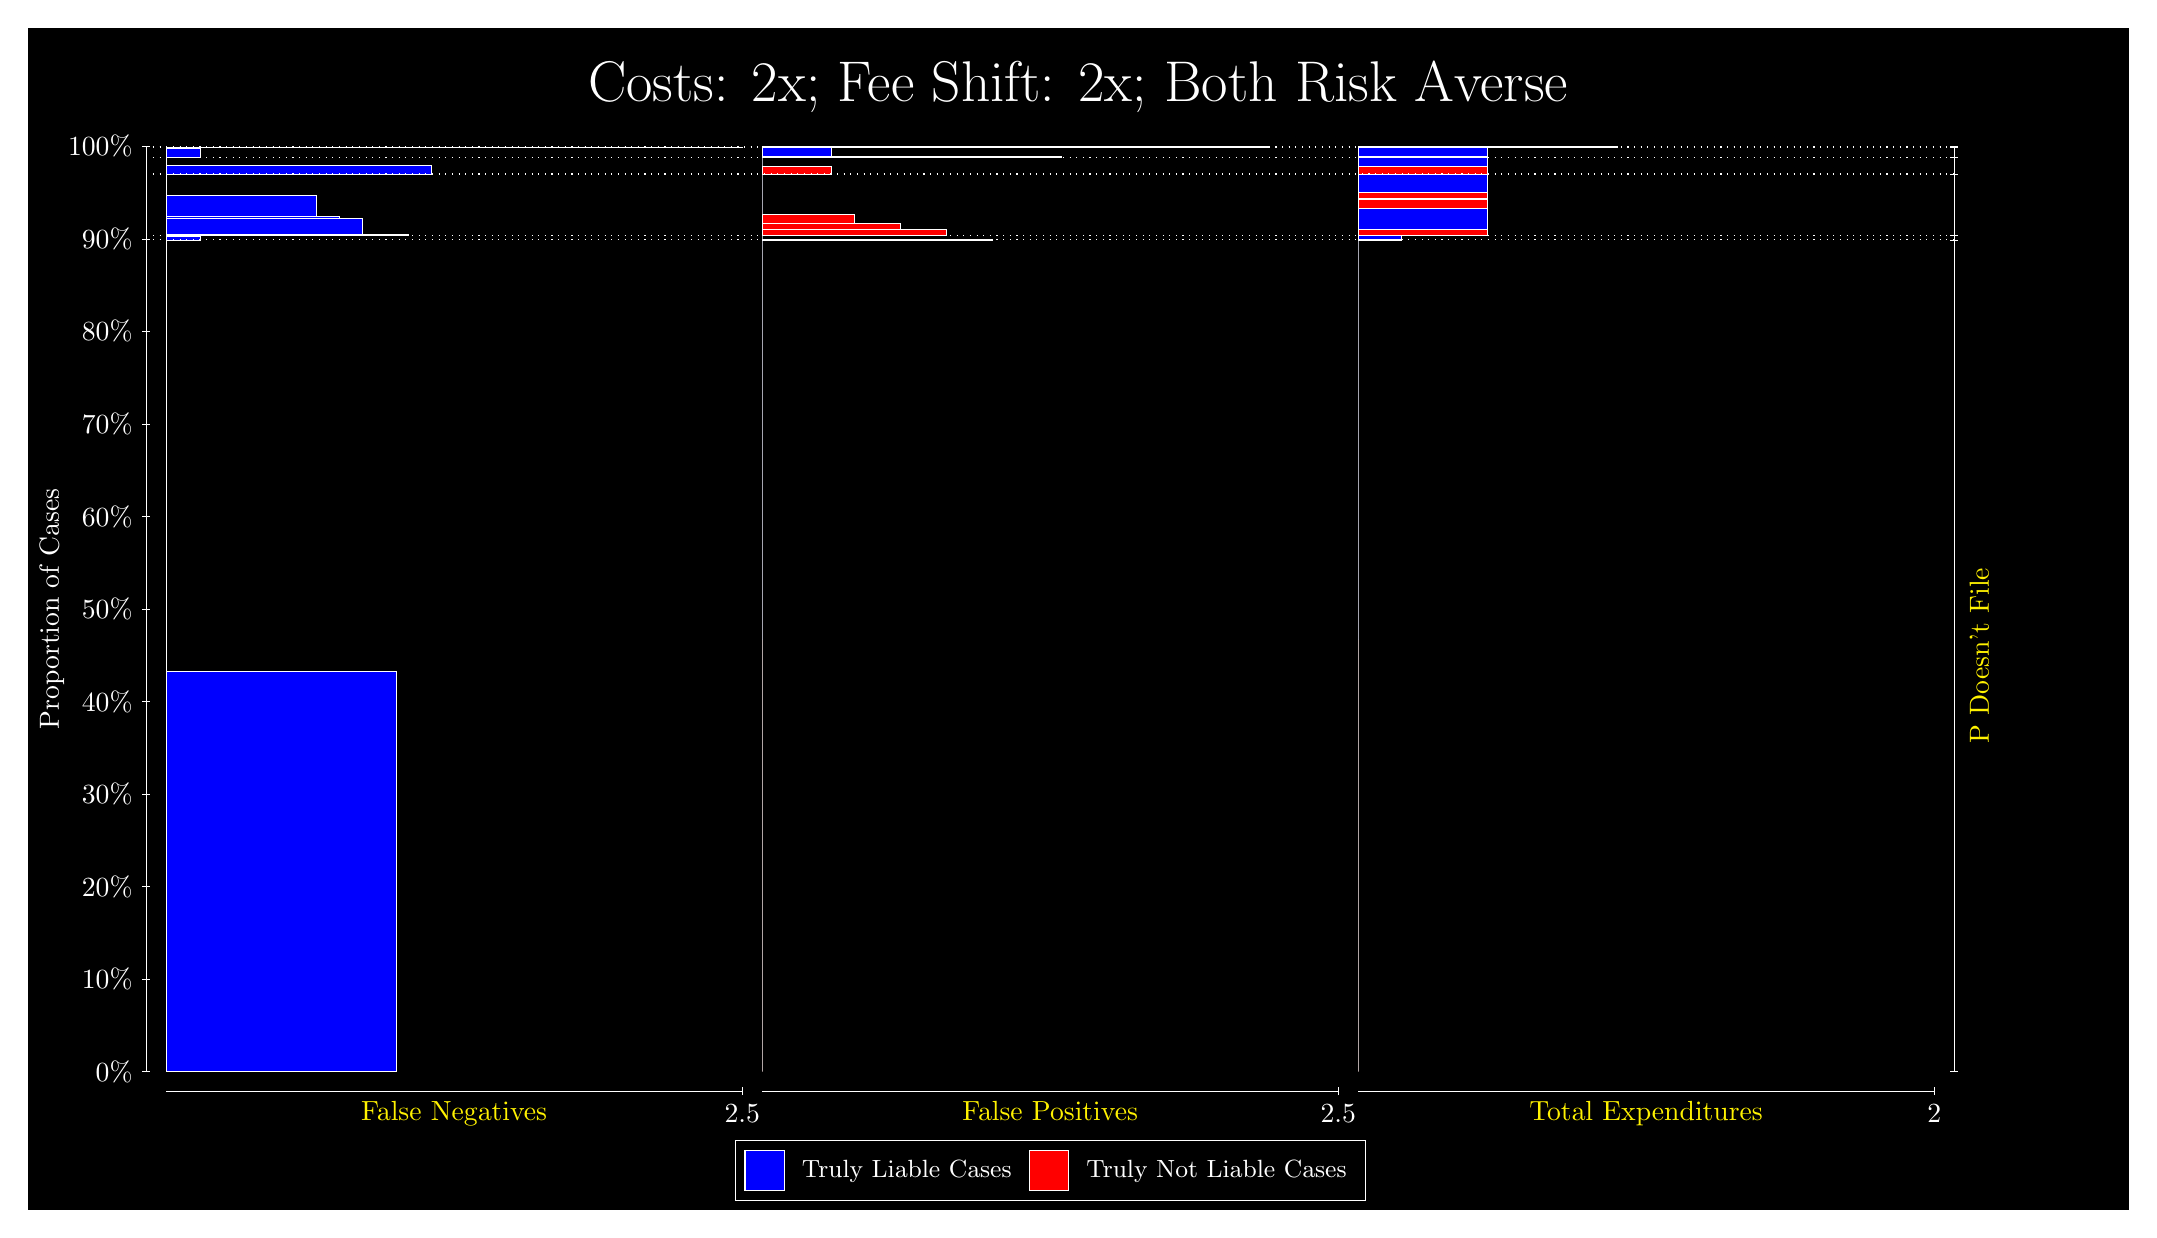
\begin{tikzpicture}
\draw[fill=black] (0,0) rectangle (26.667,15);
\draw[text=white] (0,13.5) rectangle (26.667,15) node[midway] {\huge Costs: 2x; Fee Shift: 2x; Both Risk Averse};
\draw[white, very thin] (1.5,1.75) -- (1.5,13.5);
\node[rotate=90, text=white, anchor=center] at (0.3, 7.625) {Proportion of Cases};
\draw[white, very thin] (1.45,1.75) -- (1.55,1.75);
\node[text=white, anchor=east] at (1.45, 1.75) {0\%};
\draw[white, very thin] (1.45,2.925) -- (1.55,2.925);
\node[text=white, anchor=east] at (1.45, 2.925) {10\%};
\draw[white, very thin] (1.45,4.1) -- (1.55,4.1);
\node[text=white, anchor=east] at (1.45, 4.1) {20\%};
\draw[white, very thin] (1.45,5.275) -- (1.55,5.275);
\node[text=white, anchor=east] at (1.45, 5.275) {30\%};
\draw[white, very thin] (1.45,6.45) -- (1.55,6.45);
\node[text=white, anchor=east] at (1.45, 6.45) {40\%};
\draw[white, very thin] (1.45,7.625) -- (1.55,7.625);
\node[text=white, anchor=east] at (1.45, 7.625) {50\%};
\draw[white, very thin] (1.45,8.8) -- (1.55,8.8);
\node[text=white, anchor=east] at (1.45, 8.8) {60\%};
\draw[white, very thin] (1.45,9.975) -- (1.55,9.975);
\node[text=white, anchor=east] at (1.45, 9.975) {70\%};
\draw[white, very thin] (1.45,11.15) -- (1.55,11.15);
\node[text=white, anchor=east] at (1.45, 11.15) {80\%};
\draw[white, very thin] (1.45,12.325) -- (1.55,12.325);
\node[text=white, anchor=east] at (1.45, 12.325) {90\%};
\draw[white, very thin] (1.45,13.5) -- (1.55,13.5);
\node[text=white, anchor=east] at (1.45, 13.5) {100\%};

\draw[white, very thin] (24.457,1.75) -- (24.457,13.5);
\draw[white, very thin] (24.407,1.75) -- (24.507,1.75);
\node[anchor=west] at (24.407, 1.75) {};
\draw[white, very thin] (24.407,12.313) -- (24.507,12.313);
\node[anchor=west] at (24.407, 12.313) {};
\draw[white, very thin] (24.407,12.367) -- (24.507,12.367);
\node[anchor=west] at (24.407, 12.367) {};
\draw[white, very thin] (24.407,13.148) -- (24.507,13.148);
\node[anchor=west] at (24.407, 13.148) {};
\draw[white, very thin] (24.407,13.355) -- (24.507,13.355);
\node[anchor=west] at (24.407, 13.355) {};
\draw[white, very thin] (24.407,13.492) -- (24.507,13.492);
\node[anchor=west] at (24.407, 13.492) {};
\draw[white, very thin] (24.407,13.494) -- (24.507,13.494);
\node[anchor=west] at (24.407, 13.494) {};
\draw[white, very thin] (24.407,13.5) -- (24.507,13.5);
\node[anchor=west] at (24.407, 13.5) {};

\draw[white, very thin, fill=blue] (1.75,1.75) rectangle (4.6775,6.8315);
\draw[white, very thin, fill=red] (1.75,6.8315) rectangle (1.75,12.313);
\draw[white, very thin, fill=blue] (1.75,12.313) rectangle (2.1891,12.361);
\draw[white, very thin, fill=red] (1.75,12.361) rectangle (1.75,12.367);
\draw[white, very thin, fill=blue] (1.75,12.367) rectangle (4.8239,12.385);
\draw[white, very thin, fill=blue] (1.75,12.385) rectangle (4.2384,12.581);
\draw[white, very thin, fill=blue] (1.75,12.581) rectangle (3.9457,12.617);
\draw[white, very thin, fill=blue] (1.75,12.617) rectangle (3.6529,12.877);
\draw[white, very thin, fill=red] (1.75,12.877) rectangle (1.75,13.148);
\draw[white, very thin, fill=blue] (1.75,13.148) rectangle (5.1167,13.253);
\draw[white, very thin, fill=red] (1.75,13.253) rectangle (1.75,13.355);
\draw[white, very thin, fill=blue] (1.75,13.355) rectangle (2.1891,13.479);
\draw[white, very thin, fill=red] (1.75,13.479) rectangle (1.75,13.492);
\draw[white, very thin, fill=blue] (1.75,13.492) rectangle (9.0689,13.493);
\draw[white, very thin, fill=red] (1.75,13.493) rectangle (1.75,13.494);
\draw[white, very thin, fill=red] (1.75,13.494) rectangle (1.75,13.496);
\draw[white, very thin, fill=blue] (1.75,13.496) rectangle (1.75,13.5);
\draw[white, very thin, fill=red] (9.3189,1.75) rectangle (9.3189,7.2314);
\draw[white, very thin, fill=blue] (9.3189,7.2314) rectangle (9.3189,12.313);
\draw[white, very thin, fill=red] (9.3189,12.313) rectangle (12.246,12.318);
\draw[white, very thin, fill=blue] (9.3189,12.318) rectangle (9.3189,12.367);
\draw[white, very thin, fill=red] (9.3189,12.367) rectangle (11.661,12.447);
\draw[white, very thin, fill=red] (9.3189,12.447) rectangle (11.368,12.45);
\draw[white, very thin, fill=red] (9.3189,12.45) rectangle (11.075,12.521);
\draw[white, very thin, fill=red] (9.3189,12.521) rectangle (10.49,12.637);
\draw[white, very thin, fill=blue] (9.3189,12.637) rectangle (9.3189,13.148);
\draw[white, very thin, fill=red] (9.3189,13.148) rectangle (10.197,13.25);
\draw[white, very thin, fill=blue] (9.3189,13.25) rectangle (9.3189,13.355);
\draw[white, very thin, fill=red] (9.3189,13.355) rectangle (13.125,13.368);
\draw[white, very thin, fill=blue] (9.3189,13.368) rectangle (10.197,13.492);
\draw[white, very thin, fill=red] (9.3189,13.492) rectangle (9.3189,13.493);
\draw[white, very thin, fill=blue] (9.3189,13.493) rectangle (9.3189,13.494);
\draw[white, very thin, fill=red] (9.3189,13.494) rectangle (15.759,13.496);
\draw[white, very thin, fill=blue] (9.3189,13.496) rectangle (12.832,13.5);
\draw[white, very thin, fill=red] (16.888,1.75) rectangle (16.888,7.2314);
\draw[white, very thin, fill=blue] (16.888,7.2314) rectangle (16.888,12.313);
\draw[white, very thin, fill=red] (16.888,12.313) rectangle (17.437,12.318);
\draw[white, very thin, fill=blue] (16.888,12.318) rectangle (17.437,12.367);
\draw[white, very thin, fill=red] (16.888,12.367) rectangle (18.534,12.447);
\draw[white, very thin, fill=blue] (16.888,12.447) rectangle (18.534,12.707);
\draw[white, very thin, fill=red] (16.888,12.707) rectangle (18.534,12.823);
\draw[white, very thin, fill=blue] (16.888,12.823) rectangle (18.534,12.841);
\draw[white, very thin, fill=red] (16.888,12.841) rectangle (18.534,12.915);
\draw[white, very thin, fill=blue] (16.888,12.915) rectangle (18.534,13.148);
\draw[white, very thin, fill=red] (16.888,13.148) rectangle (18.534,13.25);
\draw[white, very thin, fill=blue] (16.888,13.25) rectangle (18.534,13.355);
\draw[white, very thin, fill=red] (16.888,13.355) rectangle (18.534,13.368);
\draw[white, very thin, fill=blue] (16.888,13.368) rectangle (18.534,13.492);
\draw[white, very thin, fill=red] (16.888,13.492) rectangle (20.181,13.493);
\draw[white, very thin, fill=blue] (16.888,13.493) rectangle (20.181,13.494);
\draw[white, very thin, fill=red] (16.888,13.494) rectangle (20.181,13.496);
\draw[white, very thin, fill=blue] (16.888,13.496) rectangle (20.181,13.5);
\draw[white, dotted] (1.5,12.313) -- (24.457,12.313);
\draw[white, dotted] (1.5,12.367) -- (24.457,12.367);
\draw[white, dotted] (1.5,13.148) -- (24.457,13.148);
\draw[white, dotted] (1.5,13.355) -- (24.457,13.355);
\draw[white, dotted] (1.5,13.492) -- (24.457,13.492);
\draw[white, dotted] (1.5,13.494) -- (24.457,13.494);
\draw[white, very thin] (1.75,1.5) -- (9.0689,1.5);
\node[text=yellow, anchor=north] at (5.4094, 1.5) {False Negatives};
\draw[white, very thin] (9.0689,1.45) -- (9.0689,1.55);
\node[text=white, anchor=north] at (9.0689, 1.45) {2.5};

\draw[white, very thin] (9.3189,1.5) -- (16.638,1.5);
\node[text=yellow, anchor=north] at (12.978, 1.5) {False Positives};
\draw[white, very thin] (16.638,1.45) -- (16.638,1.55);
\node[text=white, anchor=north] at (16.638, 1.45) {2.5};

\draw[white, very thin] (16.888,1.5) -- (24.207,1.5);
\node[text=yellow, anchor=north] at (20.547, 1.5) {Total Expenditures};
\draw[white, very thin] (24.207,1.45) -- (24.207,1.55);
\node[text=white, anchor=north] at (24.207, 1.45) {2};

\node[text=yellow, centered, rotate=90] at (24.777, 7.0314) {P Doesn't File};







\draw (12.978300999999998,1.5) node[draw=none] (baseCoordinate) {};
\begin{scope}[align=center]
        \matrix[scale=0.5, draw=white, below=0.5cm of baseCoordinate, nodes={draw}, column sep=0.1cm]{
            \node[rectangle, draw, minimum width=0.5cm, minimum height=0.5cm, fill=blue] {}; &
            \node[draw=none, font=\small, text=white] (B) {Truly Liable Cases}; &
            \node[rectangle, draw, minimum width=0.5cm, minimum height=0.5cm, fill=red] {}; &
            \node[draw=none, font=\small, text=white] (B) {Truly Not Liable Cases}; \\
            };
\end{scope}

\end{tikzpicture}
\end{document}